\section{Sampling resources on the original duration-dependent scenarios}\label{sec:budget}
This is an earlier, separate resource experiment. It holds the trained models fixed and changes only the number of generated walks, using the original duration-dependent scenarios without the later step-24 rule. The two scenarios, labeled Weibull and ReLU, differ in the covariate map and covariate distribution; the Weibull scenario is the one described in Section~2 of the main text, and the label refers to that scenario, not to the Weibull-MLP direct model. The direct comparators are the Lite implementations.
\begin{center}\begin{minipage}{\textwidth}\centering
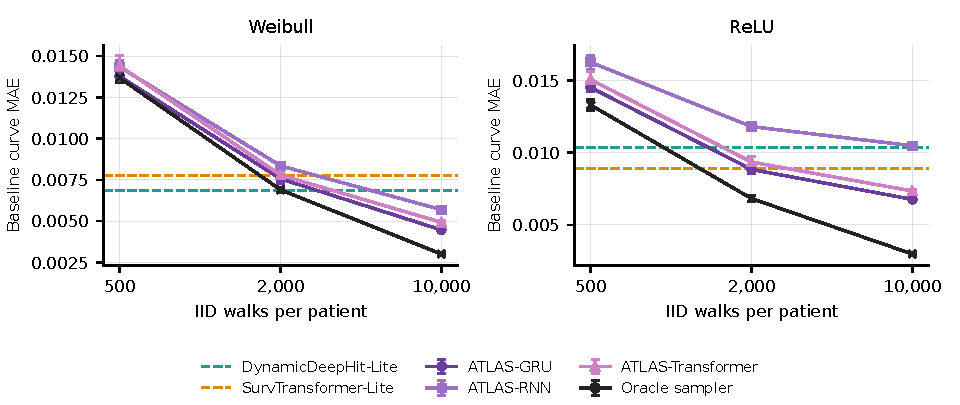
\includegraphics[width=\textwidth]{atlas_budget_baseline.pdf}
\captionof{figure}{Resource study without the step-24 rule. Baseline MAE against deterministic references, using fixed previously trained checkpoints and five IID sampling seeds. Error bars are one seed standard deviation, and dashed lines are the fixed direct predictions.}
\end{minipage}\end{center}

Increasing the IID budget reduces mean MAE in all 24 ATLAS scenario--landmark combinations, from 500 to 2,000 and again to 10,000 samples. The oracle-sampler error falls from roughly 0.0133 to 0.0142 at 500 down to 0.00296 to 0.00311 at 10,000. So a substantial share of the low-budget error is numerical. That does not mean fitted-model error disappears as sampling increases.

In the Weibull scenario at baseline, the GRU, RNN, and Transformer errors fall from 0.01377, 0.01434, and 0.01440 to 0.00447, 0.00569, and 0.00493. All three then beat DynamicDeepHit-Lite (0.00686) and SurvTransformer-Lite (0.00777). In other words, increasing prediction resources alone reverses those baseline mean-MAE comparisons, without any retraining.

The ReLU scenario supplies a useful counterexample. At 10,000 samples the GRU (0.00677) and Transformer (0.00735) beat both direct comparators, but the RNN (0.01048) remains above SurvTransformer-Lite (0.00889) and DynamicDeepHit-Lite (0.01035). At the tested nonzero landmarks, all three ATLAS models lead the two restricted direct comparators, though as before this involves different input information. Full budgets, landmarks, and variance diagnostics appear in Section~\ref{app:budgetresults}.

The single-covariate study in the main text uses a different cohort and checkpoints fitted for that process, later augmented with the history-aware comparators. Its baseline advantage should not be read as a controlled consequence of adding the hard rule alone. The resource study also replaces the earlier Monte Carlo reference with a deterministic one, so its absolute scores need not reproduce older tables computed against 2,000-trajectory reference estimates.

\clearpage
\subsection{Complete sampling-resource results}\label{app:budgetresults}
This separate study uses the original duration-dependent ramp with the step-20 change and no added step-24 deterministic override. Checkpoints, patients and reference curves are fixed across budgets. Each entry is mean curve MAE across five IID sampling seeds. All 24 ATLAS rows improve monotonically across the three budgets. ``Oracle'' is the true-generator sampler, not a fitted method.
\small
\begin{longtable}{llrrrr}
\caption{Complete sampling-resource results, mean curve MAE at each IID walk budget.}\label{tab:budgetall}\\
\toprule Scenario & Model & $L$ & $M=500$ & $M=2000$ & $M=10000$\\\midrule\endfirsthead
\toprule Scenario & Model & $L$ & $M=500$ & $M=2000$ & $M=10000$\\\midrule\endhead
ReLU & ATLAS-GRU & 0 & 0.014518 & 0.008841 & 0.006769 \\
ReLU & ATLAS-RNN & 0 & 0.016263 & 0.011810 & 0.010484 \\
ReLU & ATLAS-Transformer & 0 & 0.015063 & 0.009355 & 0.007348 \\
ReLU & Oracle & 0 & 0.013307 & 0.006825 & 0.002985 \\
ReLU & ATLAS-GRU & 10 & 0.014247 & 0.008761 & 0.006089 \\
ReLU & ATLAS-RNN & 10 & 0.016386 & 0.011745 & 0.010171 \\
ReLU & ATLAS-Transformer & 10 & 0.015216 & 0.009460 & 0.007468 \\
ReLU & Oracle & 10 & 0.013598 & 0.006749 & 0.003088 \\
ReLU & ATLAS-GRU & 15 & 0.014179 & 0.007618 & 0.004774 \\
ReLU & ATLAS-RNN & 15 & 0.016224 & 0.010833 & 0.008807 \\
ReLU & ATLAS-Transformer & 15 & 0.015783 & 0.009693 & 0.007584 \\
ReLU & Oracle & 15 & 0.014118 & 0.006693 & 0.003040 \\
ReLU & ATLAS-GRU & 20 & 0.014101 & 0.007697 & 0.005037 \\
ReLU & ATLAS-RNN & 20 & 0.015506 & 0.010321 & 0.008430 \\
ReLU & ATLAS-Transformer & 20 & 0.014544 & 0.009720 & 0.007861 \\
ReLU & Oracle & 20 & 0.013414 & 0.006423 & 0.003024 \\
Weibull & ATLAS-GRU & 0 & 0.013768 & 0.007565 & 0.004467 \\
Weibull & ATLAS-RNN & 0 & 0.014339 & 0.008350 & 0.005694 \\
Weibull & ATLAS-Transformer & 0 & 0.014399 & 0.007788 & 0.004929 \\
Weibull & Oracle & 0 & 0.013677 & 0.006900 & 0.003010 \\
Weibull & ATLAS-GRU & 10 & 0.014386 & 0.008124 & 0.005239 \\
Weibull & ATLAS-RNN & 10 & 0.015153 & 0.009876 & 0.007502 \\
Weibull & ATLAS-Transformer & 10 & 0.015230 & 0.009429 & 0.006946 \\
Weibull & Oracle & 10 & 0.013939 & 0.006827 & 0.003113 \\
Weibull & ATLAS-GRU & 15 & 0.014626 & 0.009031 & 0.006469 \\
Weibull & ATLAS-RNN & 15 & 0.015845 & 0.010777 & 0.008936 \\
Weibull & ATLAS-Transformer & 15 & 0.015952 & 0.010113 & 0.008064 \\
Weibull & Oracle & 15 & 0.014236 & 0.006960 & 0.003054 \\
Weibull & ATLAS-GRU & 20 & 0.015615 & 0.010581 & 0.009266 \\
Weibull & ATLAS-RNN & 20 & 0.015003 & 0.010222 & 0.008346 \\
Weibull & ATLAS-Transformer & 20 & 0.013618 & 0.007538 & 0.004785 \\
Weibull & Oracle & 20 & 0.013597 & 0.006617 & 0.002957 \\
\bottomrule\end{longtable}\normalsize
The archive also records seed SD, ensemble-curve MAE, pointwise sampling variance, and an exact finite-replicate MSE identity.  For $R$ prediction replicates with mean curve $\bar S$, the averaged squared error satisfies
\[
 \frac1R\sum_{r=1}^R\|\widehat S_r-S^*\|^2
 =\|\bar S-S^*\|^2+\frac1R\sum_{r=1}^R\|\widehat S_r-\bar S\|^2,
\]
where the norm averages over patients and scored horizons. The mean-curve term still contains finite-replicate Monte Carlo error and is not pure model bias. The raw variance and comparison tables ship with the source. Baseline references here are deterministic, whereas the older local runs used 2,000 simulated reference trajectories, so their absolute MAEs are not directly interchangeable.
